% !TeX spellcheck = en_US
\section{Problem 4}
Problem 4 depends on Problem 3's neural network, but it is executed using different initial values.

\begin{figure}[htpb]
	\centering
	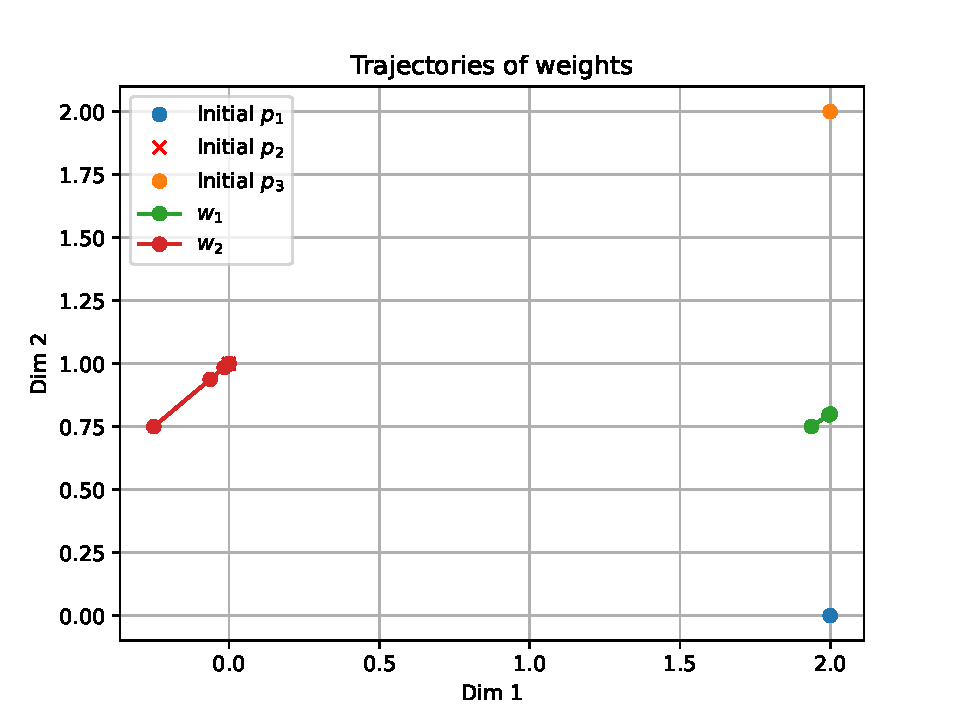
\includegraphics[width=0.5\linewidth]{../Problem 4/prob4_weights_over_epoch.pdf}
	\caption{Trajectory of weights during training.}
	\label{fig:prob4_weight_trajectory}
\end{figure}

In figure~\ref{fig:prob4_weight_trajectory}, the weight trajectory can be seen.
Based on the final weight positions after training, we can infer the clustering of the three vectors as follows:\\

\underline{Weight $W_1$} has moved towards and is located at the coordinates ($2.0, 0.8$), which is close to both $p_1$ ($2, 0$) and $p_3$ ($2, 2$). Given that these points are close to the input space and $W_1$ is approximately at the mean of the vertical component of $p_1$ and $p_3$, it suggests that $W_1$ would be the winning neuron for inputs similar to $p_1$ and $p_3$ in a larger number of iterations. This means that both $p_1$ and $p_3$ would be clustered together.

\underline{Weight $W_2$} has moved to a position very close to $p2$ ($0, 1$), which is at the coordinates (\num{-9.53674316e-07}, \num{9.99999046e-01}) $\approx$ ($0,1$). This indicates that $W_2$ has adjusted to represent input $p_2$.\\

Therefore, if the network continues to be trained for a larger number of iterations, the three vectors are likely to be clustered into two groups:

\begin{itemize}
	\item Cluster 1: Inputs $p_1$ and $p_3$, represented by $W_1$.
	\item Cluster 2: Input $p_2$, represented by $W_2$.
\end{itemize}
\vspace{3mm}
